\chapter{特征融合及RLCCD框架验证}
\label{chap:fusion}
本章主要对面向代码克隆检测的多维源代码表征方法整体框架RLCCD进行介绍,同时进行实验评估及验证。具体地,RLCCD是由上述基于预训练辅助模型的Token表征学习、基于子树划分的抽象语法树表征学习、基于图过滤的程序依赖图表征学习方法三种维度融合形成并进行实现的表征方法,最后通过与SourcererCC、ASTNN、SCDetector进行对比实验以验证该框架的有效性。
\section{特征融合}
特征融合方法是指将不同来源或不同层次的特征进行组合,合并成一个比输入特征更具有判别能力的特征,该多维特征能够在低维空间中高效计算实体和关系的语义联系,提高特征的表达能力和分类效果,有利于下游代码克隆检测任务的学习。

因此,经过第\ref{chap:Token}、\ref{chap:AST}、\ref{chap:PDG}章的表征学习,得到三种维度的特征向量:属性特性$V^{Token}$、结构特征$V^{AST}$、语义特征$V^{PDG}$。上述三种表征方式得到的特征向量通常具有信息互补性,且不同维度的特征是代码表示的平行语料,具有信息等价性,因此,本文提出了基于多模态学习的特征融合方法,将三个维度的特征向量通过特征融合生成多维表示。然后将多维表示送入单层线性网络。本文设计了两个特征融合方式:特征连接(Feature concatenation)和特征加法(Feature addition),如下图\ref{fig:concat_add}所示。

\begin{figure}[H]
  \centering
  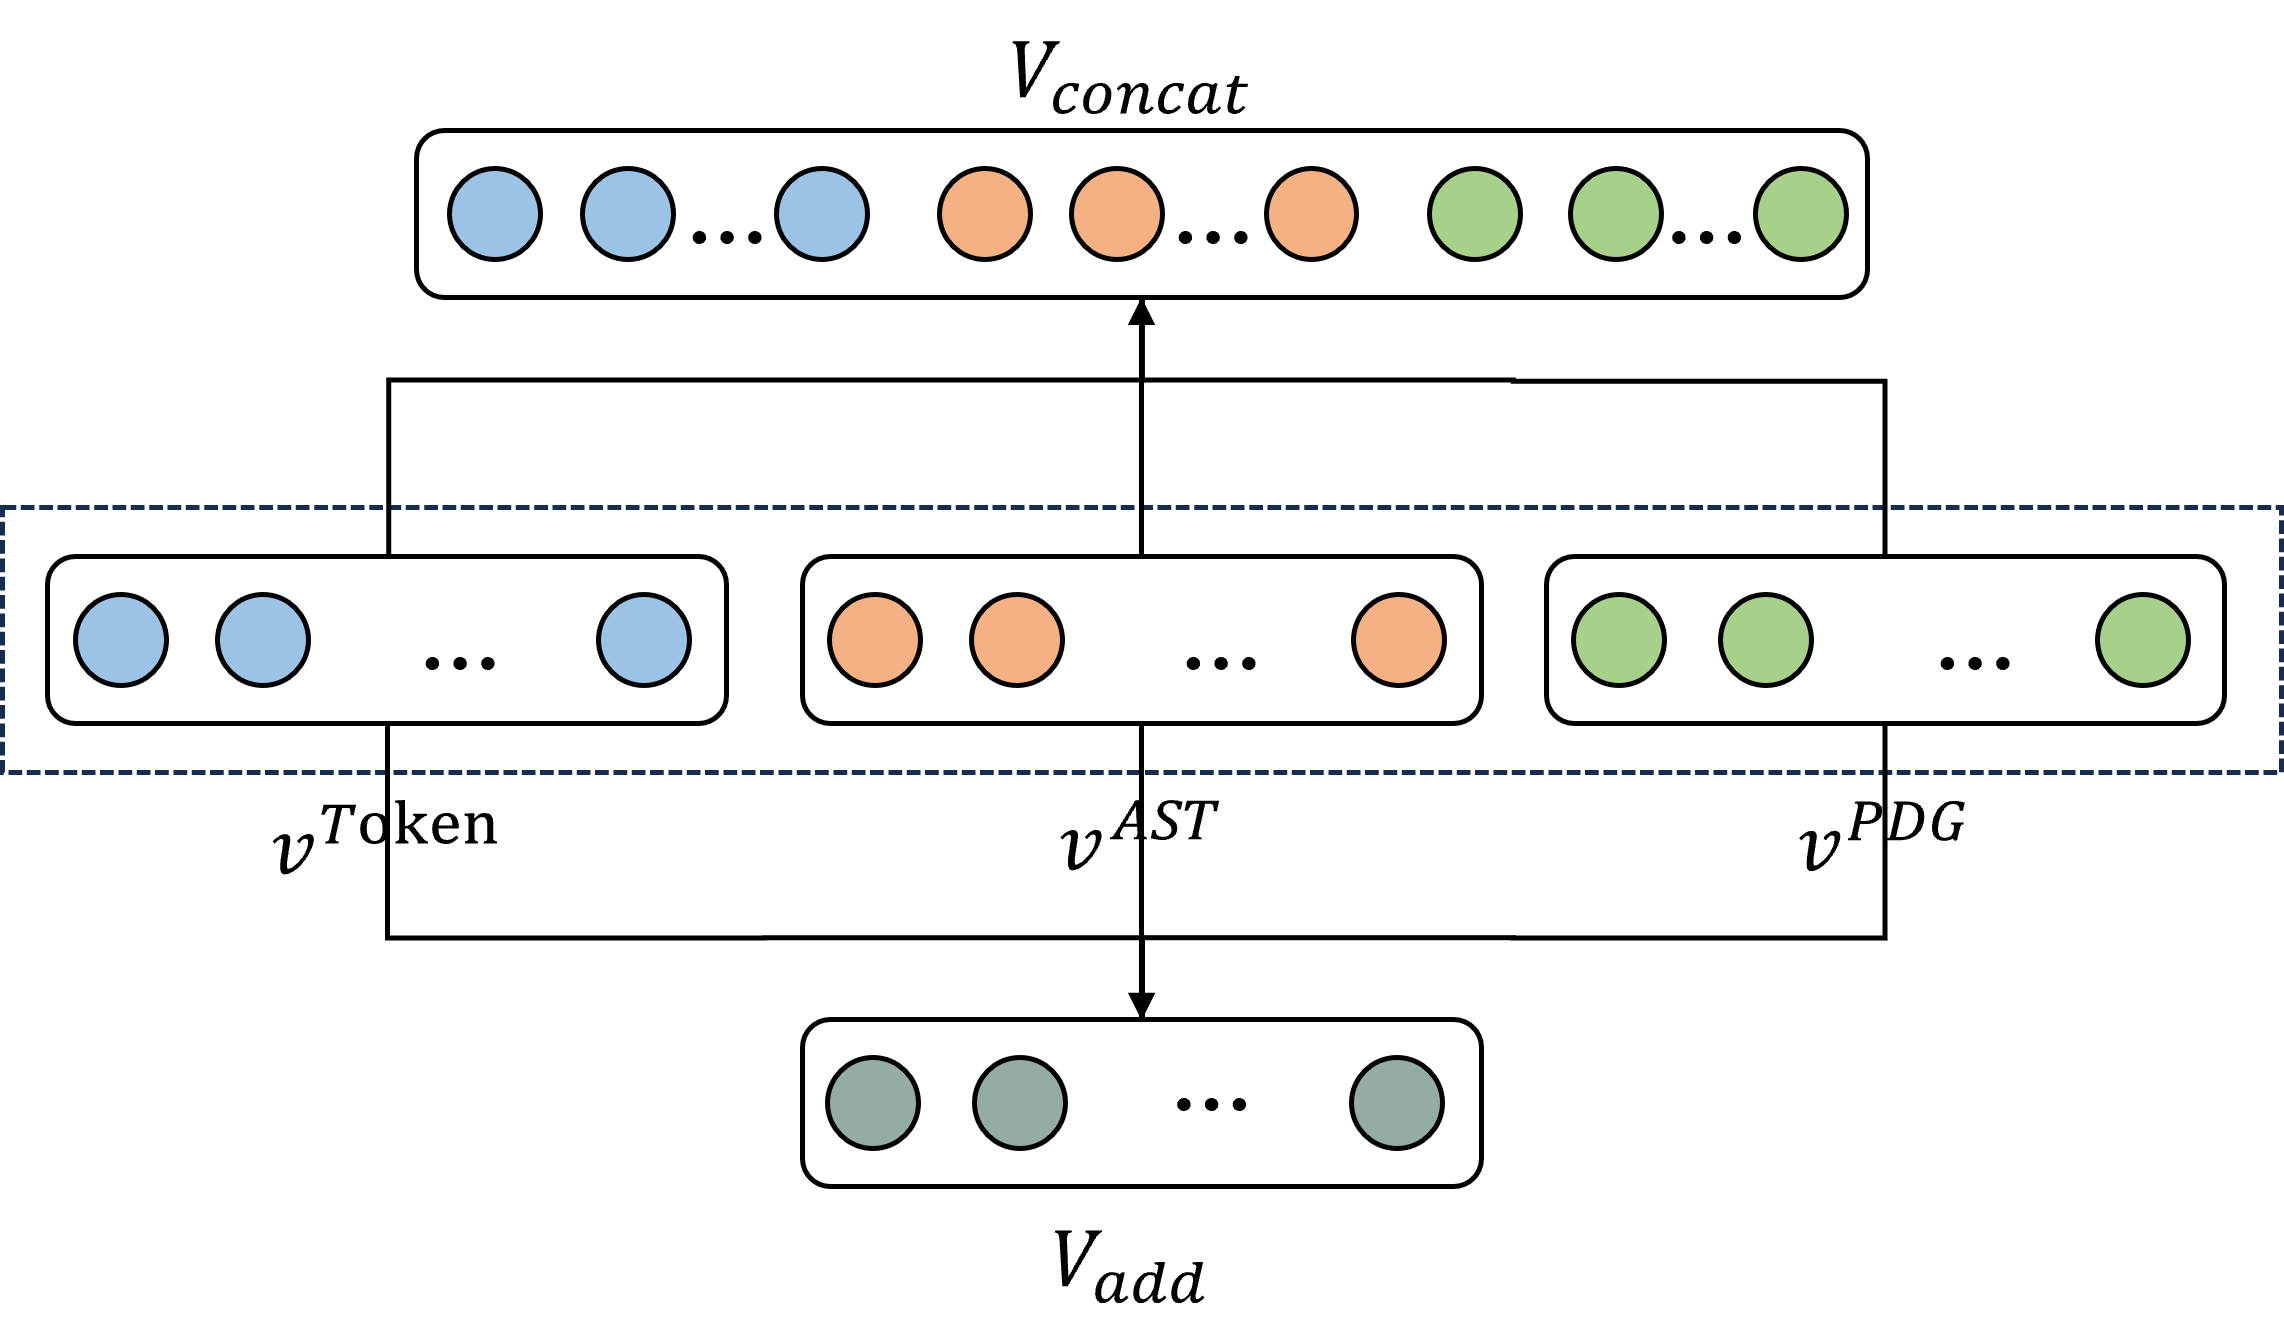
\includegraphics[width=0.55\textwidth]{figures/concat_add.png}
  \caption{特征融合方法}\label{fig:concat_add}
\end{figure}

其中特征连接是指直接将两个特征张量在某个维度上连接在一起,生成一个更大的张量。例如两个输入特征x和y的维数若为p和q,输出特征z的维数为p+q。在连接时,采取串联策略,两个张量的维度必须保持一致。而特征加法是指将两个特征张量按照元素相加在一起,生成一个新的张量。采取并行策略,特征向量本身的维度并没有增加。因此可以用公式\ref{e6.1}表示:

\begin{equation}\label{e6.1}
  \begin{split}
    \tilde{V_{concat}} &= concat \left( V^{\text{Token}} , V^{\text{AST}} , V^{\text{PDG}}\right) \\
    \tilde{V_{add}} &= add \left( V^{\text{Token}} , V^{\text{AST}} , V^{\text{PDG}}\right) \\
    V &= W_{dt} \cdot \tilde{V} + b_{dt}
  \end{split}
\end{equation}

其中$V$表示最终的多维混合代码表示,$W_{dt}$在生成的多维混合表示中平衡属性特征、结构特征、语义特征的组成,而$b_{dt}$在训练模型时使模型偏向最终收敛。

\section{RLCCD框架验证}
本文的实验设计主要围绕以下5个方面的研究问题:

• RQ1:本文提出的预训练辅助模型策略是否优于基线方法?

• RQ2:本文提出的子树划分策略是否优于基线方法?

• RQ3:本文提出的图过滤策略能否优于基线方法?

• RQ4:本文提出的特征融合方法是否优于单维度方法?

• RQ5:本文提出的多维源代码表征学习方法与现有代码克隆检测工具相比表现如何?

在上述5个方向的研究问题中,RQ1是针对Token维度优化策略的评估,在\ref{sec:TokenExperiment}小节中已经给出;RQ2是针对抽象语法树维度优化策略的评估,在\ref{sec:ASTExperiment}小节中已经给出;RQ3是针对程序依赖图维度优化策略的评估,在\ref{sec:PDGExperiment}小节中已经给出;RQ4是针对特征融合方法进行评估;RQ5从整体工具有效性的角度开展评估。

\subsection{实验设置}
(1)系统环境

本章实验均在Ubuntu 16.04 LTS(64位)系统下进行,其系统硬件配置与\ref{subsec:Environment}所述相同。


(2)实验数据集

为了验证RLCCD的可行性与有效性,本章实验仍选用与前述\ref{subsec:Dataset}相同的数据集。

\subsection{对比工具}

为了更好地对比整个方法的实验效果,本文选取近几年来各个维度较为先进、经典开源的方法,并在相同数据集上进行了检测结果的对比,具体方法主要如表\ref{tab:tool}所示。

\begin{table}[htp]
  \centering
  \caption{代码克隆检测实验对比工具介绍} 
  \label{tab:tool}
  \renewcommand{\arraystretch}{1.1}
  \begin{tabular*}{0.8\textwidth}{@{\extracolsep{\fill}}cc}
  \toprule
    方法名称			&类型介绍		\\
  \midrule
  SourcererCC		 &基于Token的克隆检测方法 \\
  ASTNN			     &基于AST的克隆检测方法 \\
  CCSharp		     &基于PDG的克隆检测方法 \\
  SCDetector		 &基于Token、PDG的克隆检测方法 \\
  RLCCD(本文方法)	&基于Token、AST、PDG多种维度的克隆检测方法 \\
  \bottomrule
  \end{tabular*}
\end{table}

SourcererCC\cite{7886988}:SourcererCC是一种相对较新的基于token的克隆检测工具。该工具通过词袋模型,把收集的数据全部编码成词频信息,然后将代码行转换成一个由词频构成的向量,通过向量的比较获取相似度。

ASTNN\cite{8812062}:ASTNN是一种基于神经网络的源代码表示方法。它将整个抽象语法树AST分解成一系列小型语句子树,并通过捕获语句的词法和语法信息将语句子树分别编码为向量,最后采用了RNN模型生成代码片段的向量表示。ASTNN方法完整保留了抽象语法树的结构信息,能够检测到所有类型的代码克隆。

CCSharp\cite{9286111}:CCSharp是一种基于程序依赖图的代码克隆检测方法。它首先生成了源代码中函数级别的PDG,并对生成的图结构进行约简,随后进行特征向量的提取和过滤,最后应用Weisfeiler-Lehman图核算法进行图相似性比较找出代码克隆对。

SCDetector\cite{10.1145/3324884.3416562}:SCDetector一种是基于Token和图结合的方法。给定一个方法源代码,首先生成CFG,然后应用中心性分析将图转换为某些语义标记(即具有图细节的标记)。最后,这些语义标记被送到Siamese网络中,以训练模型并使用它来检测代码克隆对。

为了验证本文所提方法在克隆上的有效性,所有工具试实验结果均采用其参考文献中所提供的最好效果的参数配置,并统一在相同的实验数据集POJ104上进行对比实验。

\subsection{特征融合方法实验结果}



\begin{table}[htp]
  \centering
  \caption{特征融合方法对实验结果的影响}
  \label{tab:concat}
  \begin{tabular*}{0.9\textwidth}{@{\extracolsep{\fill}}cccc}
  \toprule
    对比			& 准确率P(\%) & 召回率R(\%) & F1值(\%)  \\ 
  \midrule
    Token维度			  & 89.78	  & 95.62	  & 92.61	   \\  
    树维度		      & 92.75	  & 87.62	  & 90.11   \\ 
    图维度			    & 89.53		& 81.71		& 85.44   \\
    add融合			   & 92.89		& 90.35		& 91.60   \\
    concat融合     	  & 93.82		& 92.27		& 93.04  \\
  \bottomrule
  \end{tabular*}
\end{table}


基于对表\ref{tab:concat}数据的分析,可以得到以下结论:(1)concat特征融合方法整体比add融合方法表现优秀。深究其原因,add操作相当于加入一种先验知识,对原始特征进行人为的特征融合。它描述的是代码特征信息量增多,但维度本身并没有增加,这种操作对最终的分类是有益的。而concat操作是特征维度的增加,而每一特征下的信息并没有增加。这意味着concat可以扩展特征的空间,让模型能够看到更多的信息和变化。通过将不同来源的特征拼接在一起,concat可以促进特征之间的交互和整合,进一步提高模型的表现,使模型同时关注图像的局部和整体信息,因此具有更好的代码克隆检测能力。


\subsection{RLCCD性能评估实验结果}

对比实验:体现框架的有效性


\begin{table}[htp]
  \centering
  \caption{RLCCD实验结果}
  \label{tab:RLCCD}
  \begin{tabular*}{0.9\textwidth}{@{\extracolsep{\fill}}cccc}
  \toprule
    对比工具		& 准确率P(\%) & 召回率R(\%) & F1值(\%)  \\ 
  \midrule
    SourcererCC		& 11.23	  & 43.52		& 17.84 \\
    ASTNN			    & 87.92		& 95.47		& 91.54 \\
    SCDetector		& 97.02	  & 81.05		& 88.32 \\
    RLCDD			    & 93.82		& 92.27		& 93.04  \\
  \bottomrule
  \end{tabular*}
\end{table}

\section{本章小结}
本章节主要对RLCCD框架进行了实验验证,以验证RLCCD的XXX能力。



